\chapter{Methodology}
\label{chap:methods}

\section{Dataset}

The dataset utilized for training our generative models and the \gls{cnn} model was obtained from the research conducted by \cite{5} called the ViC dataset. This dataset comprises 2400 images belonging to 12 different scenarios for two channels. 

Each channel in the system can be in one of four states: unused (empty), occupied by a primary user (RADAR), occupied by a secondary user (LTE), or experiencing interference (collision). Since the system involves two channels and two tiers of users, this results in 16 possible channel usage combinations. However, four of these combinations are excluded because the \gls{cbsd} is designed to operate on only one channel at a time. Therefore, the channels can exhibit 12 valid state configurations. Figure 2.1 presents the spectrograms that correspond to these 12 distinct channel states. A dataset of 2000 images was used to train the generative models, while an additional 400 images were used for training the CNN classifier.

The class names presented in Figure 2.1 will be used throughout this paper when discussing the results. Waveforms were visualized using  Short Time Fourier Transform (STFT) with a size of $64 \times 64 $ matrix.

\begin{figure}[h]
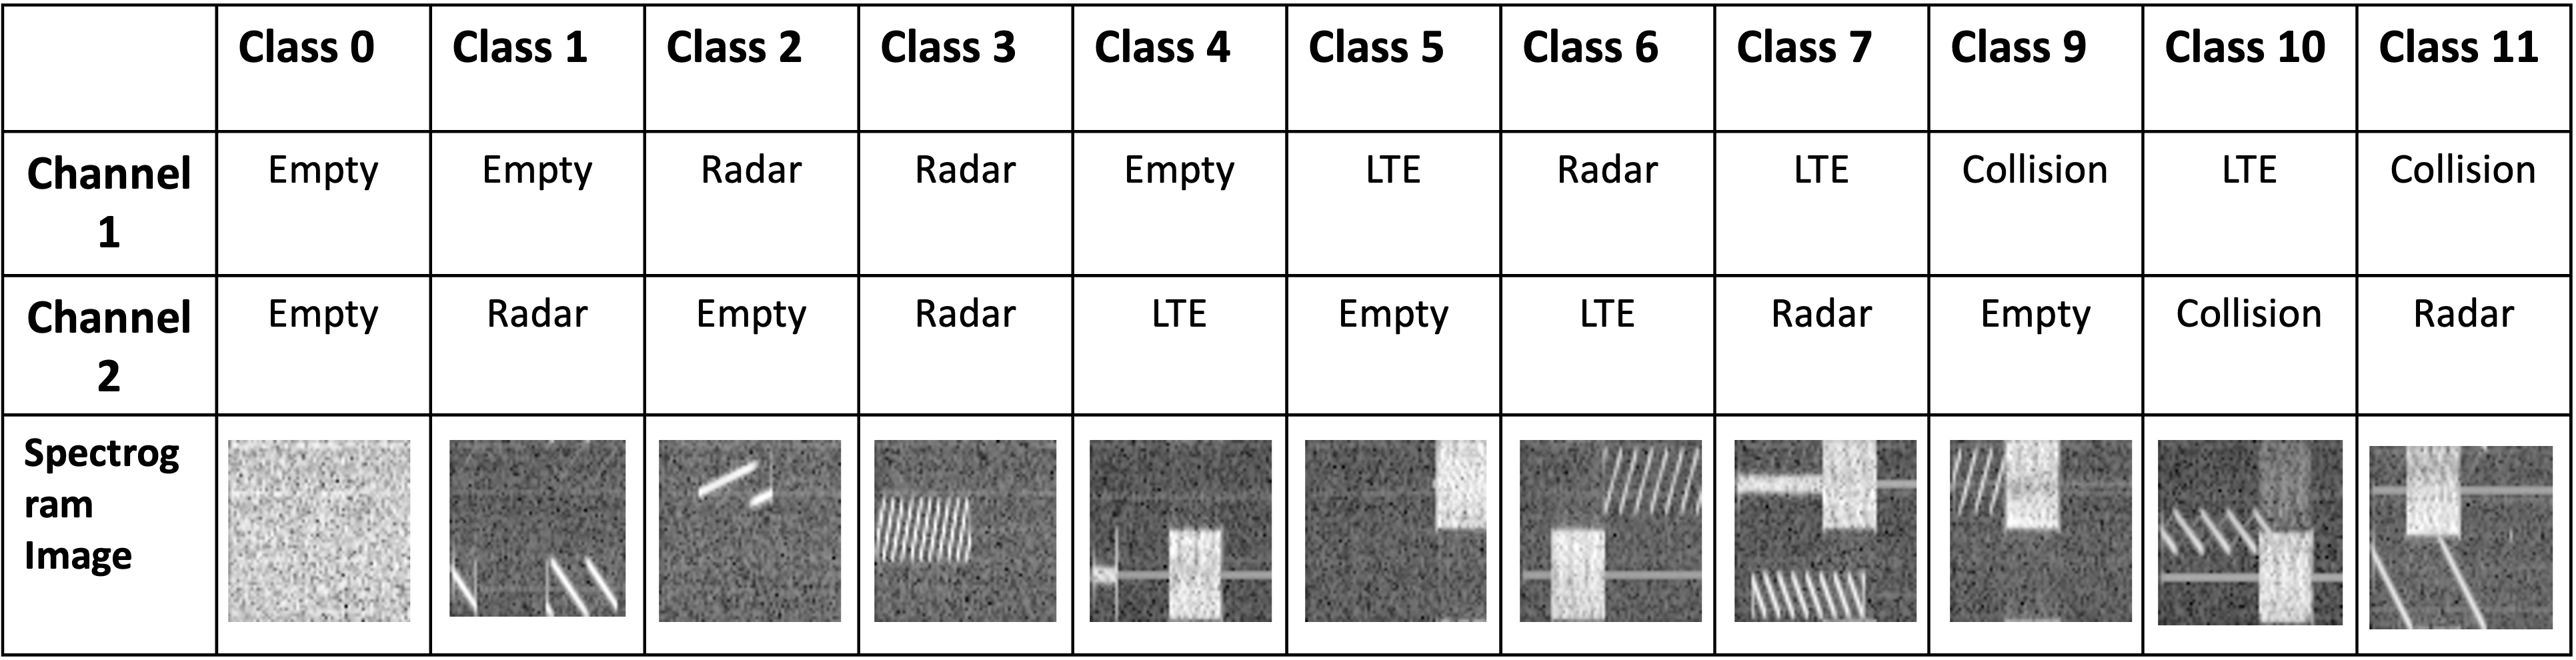
\includegraphics[width=\textwidth]{figures/classes_white_background.png}
\centering
\caption{Training ViC dataset containing the 12 classes \cite{5}}
\label{fig:training-dataset}
\centering
\end{figure}
%%%%%%%%%%%%%%%%%%%%%%%%%%%%%%%%%%%%%%%%%%%%%%%%%%%%%%%%%%%%%%%%%%%%%%%%%%%%%%%%%%%%%%%%%%%%%%%%%
\section{\gls{vq-vae}}

The \gls{vq-vae} is a generative model that combines continuous latent representations with discrete, interpretable codes by introducing a quantization mechanism. As illustrated in Figure 2.2 In \gls{vq-vae}, the encoder maps the input $x$ to a continuous latent representation $z_e(x)$ which is then quantized to the closest embedding $z_q(x)$ from a predefined discrete codebook ${e_1,e_2,...,e_k}$. This process ensures that the latent space is discrete and semantically meaningful. During training, the quantization mechanism minimizes the difference between $z_e(x)$ and $z_q(x)$ using a gradient-through approximation. The decoder then reconstructs the input $x$ from the quantized representation $z_q(x)$. The use of codebook ${e_1,e_2,...,e_k}$ enables the model to structure the latent space compactly, making it highly effective for tasks like image generation and speech synthesis. This discrete representation, denoted by $q(z|x)$, improves reconstruction quality by focusing on meaningful latent structures and allows efficient scaling for large datasets and complex generative tasks. The innovation of replacing continuous latent spaces with quantized embeddings results in a model that bridges the gap between interpretability and high-quality generation.

\begin{figure}[h]
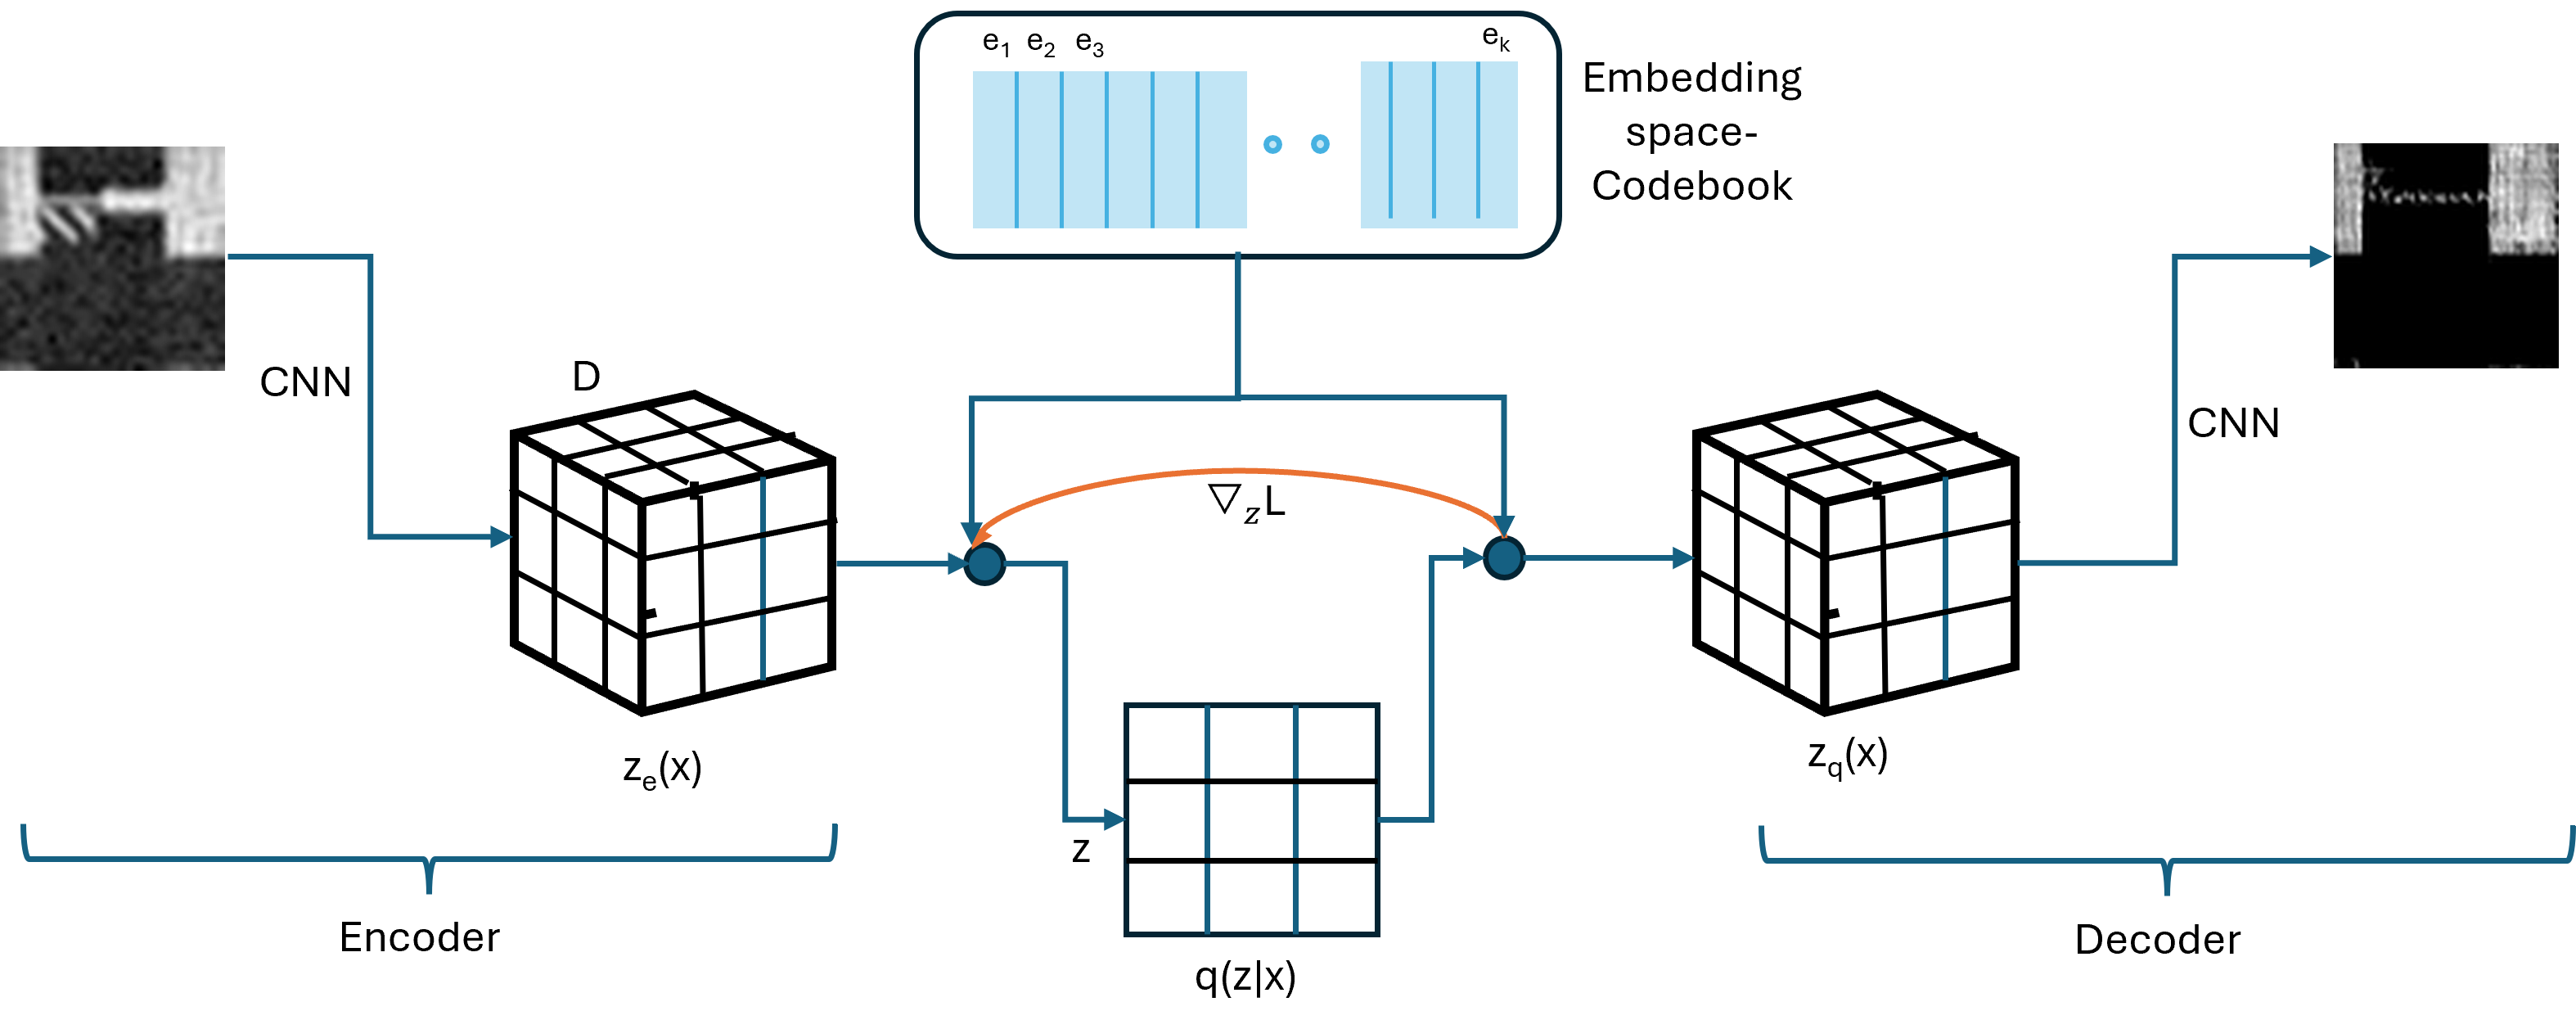
\includegraphics[width=\textwidth]{figures/vq-vae.png}
\centering
\caption{The \gls{vq-vae} architecture  }
\centering
\end{figure}


In the architecture of the conditional \gls{vq-vae} we used, the encoder is a \gls{cnn} designed to extract features from the input grayscale images.It consists of three convolutional layers that gradually decrease the spatial resolution while expanding the depth of feature maps. The encoder also incorporates a residual stack, which consists of multiple residual layers to enhance feature extraction by allowing information to bypass intermediate transformations, thereby improving gradient flow and capturing complex patterns.

After encoding, the latent representation is passed through a 1x1 convolution layer to adjust the feature dimensions to match the input requirements of the vector quantizer.  This mapping is performed using the Euclidean distance between the latent vectors and the codebook embeddings. To ensure effective learning, the vector quantizer minimizes a combination of the reconstruction loss, a codebook commitment loss, and a latent quantization loss.
The loss function can be expressed as follows:
\begin{equation}
L = \mathbb{E}[\|x - \hat{x}\|^2] + \beta \cdot \mathbb{E}[\|z_{\text{enc}} - \text{sg}(z_{\text{quant}})\|^2]
\end{equation}

where $x$ is the input image, $\hat{x}$ is the reconstructed image, $z_{\text{enc}}$ is the latent vector from the encoder, $z_{\text{quant}}$ is the quantized vector, and $\text{sg}(\cdot)$ denotes the stop-gradient operator.

The decoder is another \gls{cnn} that takes the quantized latent representations and reconstructs the original input images. It mirrors the encoder's structure, starting with a convolutional layer followed by the residual stack to refine features, and ends with transposed convolutional layers to upsample the latent representation back to the original input dimensions. The decoder ensures that the reconstructed images retain high fidelity to the input.

We implemented a conditional \gls{vq-vae} model, enabling class-specific image generation. The encoder compresses grayscale input images using three convolution layers followed by residual blocks, while the decoder mirrors this process using transposed convolutions to reconstruct the data. The quantization layer is also class-conditioned, leveraging a codebook with 512 embeddings, each of 64 dimensions. 

%%%%%%%%%%%%%%%%%%%%%%%%%%%%%%%%%%%%%%%%%%%%%%%%%%%%%%%%%%%%%%%%%%%%%%%%%%%%%%%%%%%%%%%%%%%%%%%%%
\section{\gls{gan}}

\gls{gan}s, are composed of two neural components: a generator that synthesizes data samples and a discriminator that assesses their authenticity. These two models are trained in an adversarial framework, where the generator attempts to produce data that the discriminator cannot distinguish from real data, while the discriminator learns to correctly differentiate between real and generated samples. Through this competitive training, GANs are capable of generating highly realistic images, audio, and other types of data \cite{10}. The corresponding loss functions for the generator and discriminator are expressed below. Figure 2.3 illustrates this architecture.
\begin{figure}[h]
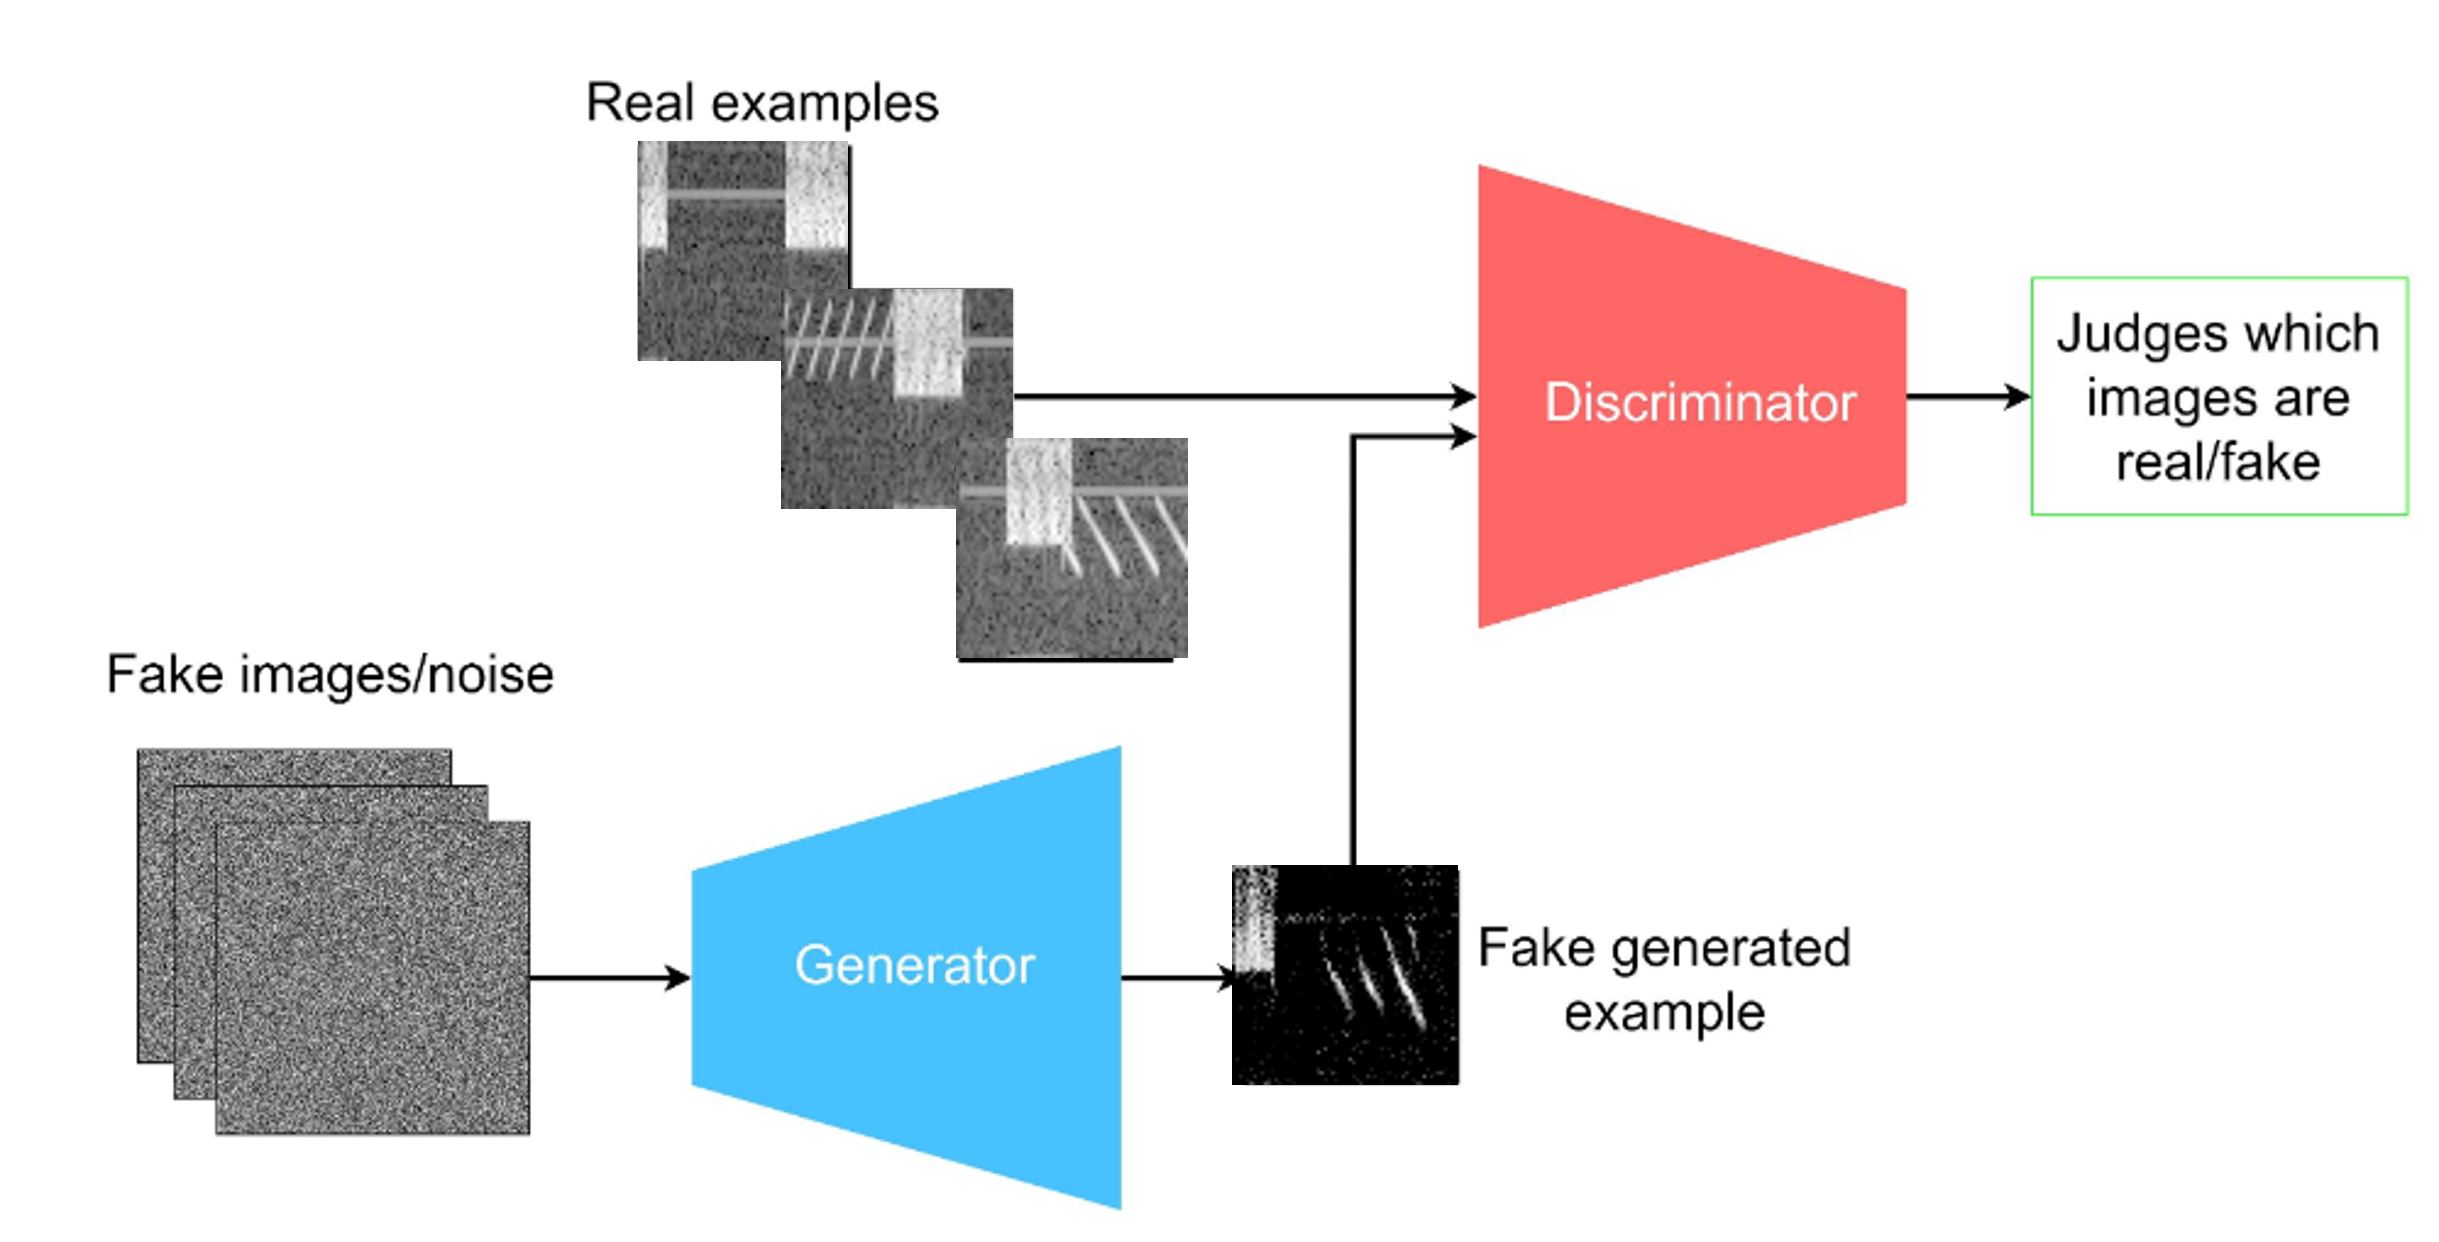
\includegraphics[width=9cm]{figures/gan.png}
\centering
\caption{The \gls{gan} architecture  }
\centering
\end{figure} 
 $L_D$ and $L_G$ are the loss functions for the Discriminator and the Generator for image $x$, respectively.
\begin{equation}
    L_D=\mathbb{E}[max(0,1 - D(x_{real}))]+\mathbb{E}[max(0,1+D(G(z_{fake})))]
\end{equation}

\begin{equation}
    L_G=\mathbb{E}[D(G(z_{fake}))]
\end{equation}

We used a conditional \gls{gan} with a Generator $\mathcal{G}$ and a Discriminator $\mathcal{D}$ which were trained simultaneously through a min-max game. For the Generator, we used an input noise vector $z$ of 100 dimensions and an embedding layer to convert class labels into embeddings with five convolution layers and ReLU activations in hidden layers. Tanh activation was used in the output layer to produce pixel values in the range [-1, 1]. In the Discriminator, five convolution layers were used to down-sample the images with Leaky ReLU activations in hidden layers. We used Sigmoid activation in the output layer to produce the probability.
\begin{figure}[h]
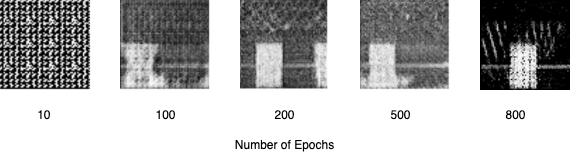
\includegraphics[width=9cm]{figures/gan training.drawio (1).png}
\centering
\caption{Spectrogram images generated by the Generator of the \gls{gan}}
\centering
\end{figure}

We generated 1200 images with 100 images per class for the twelve classes and used the pre-trained \gls{cnn} model to classify the images. 

%%%%%%%%%%%%%%%%%%%%%%%%%%%%%%%%%%%%%%%%%%%%%%%%%%%%%%%%%%%%%%%%%%%%%%%%%%%%%%%%%%%%%%%%%%%%%%%%%
\section{\gls{ddpm}}

\gls{ddpm}s are generative models designed for image generation using variational inference. They operate through a Markovian process that involves a finite sequence of steps, denoted as $T$.
The training process consists of two key phases: the forward phase, which gradually introduces noise to the data in a systematic way, and the reverse phase, where the model is trained to progressively remove the noise and reconstruct the original data.
Each step in this process acts as a denoising operation, aiming to refine the image quality progressively\cite{7}. Figure 2.5 illustrates the diffusion process of the \gls{ddpm}. 

\begin{figure}[h]
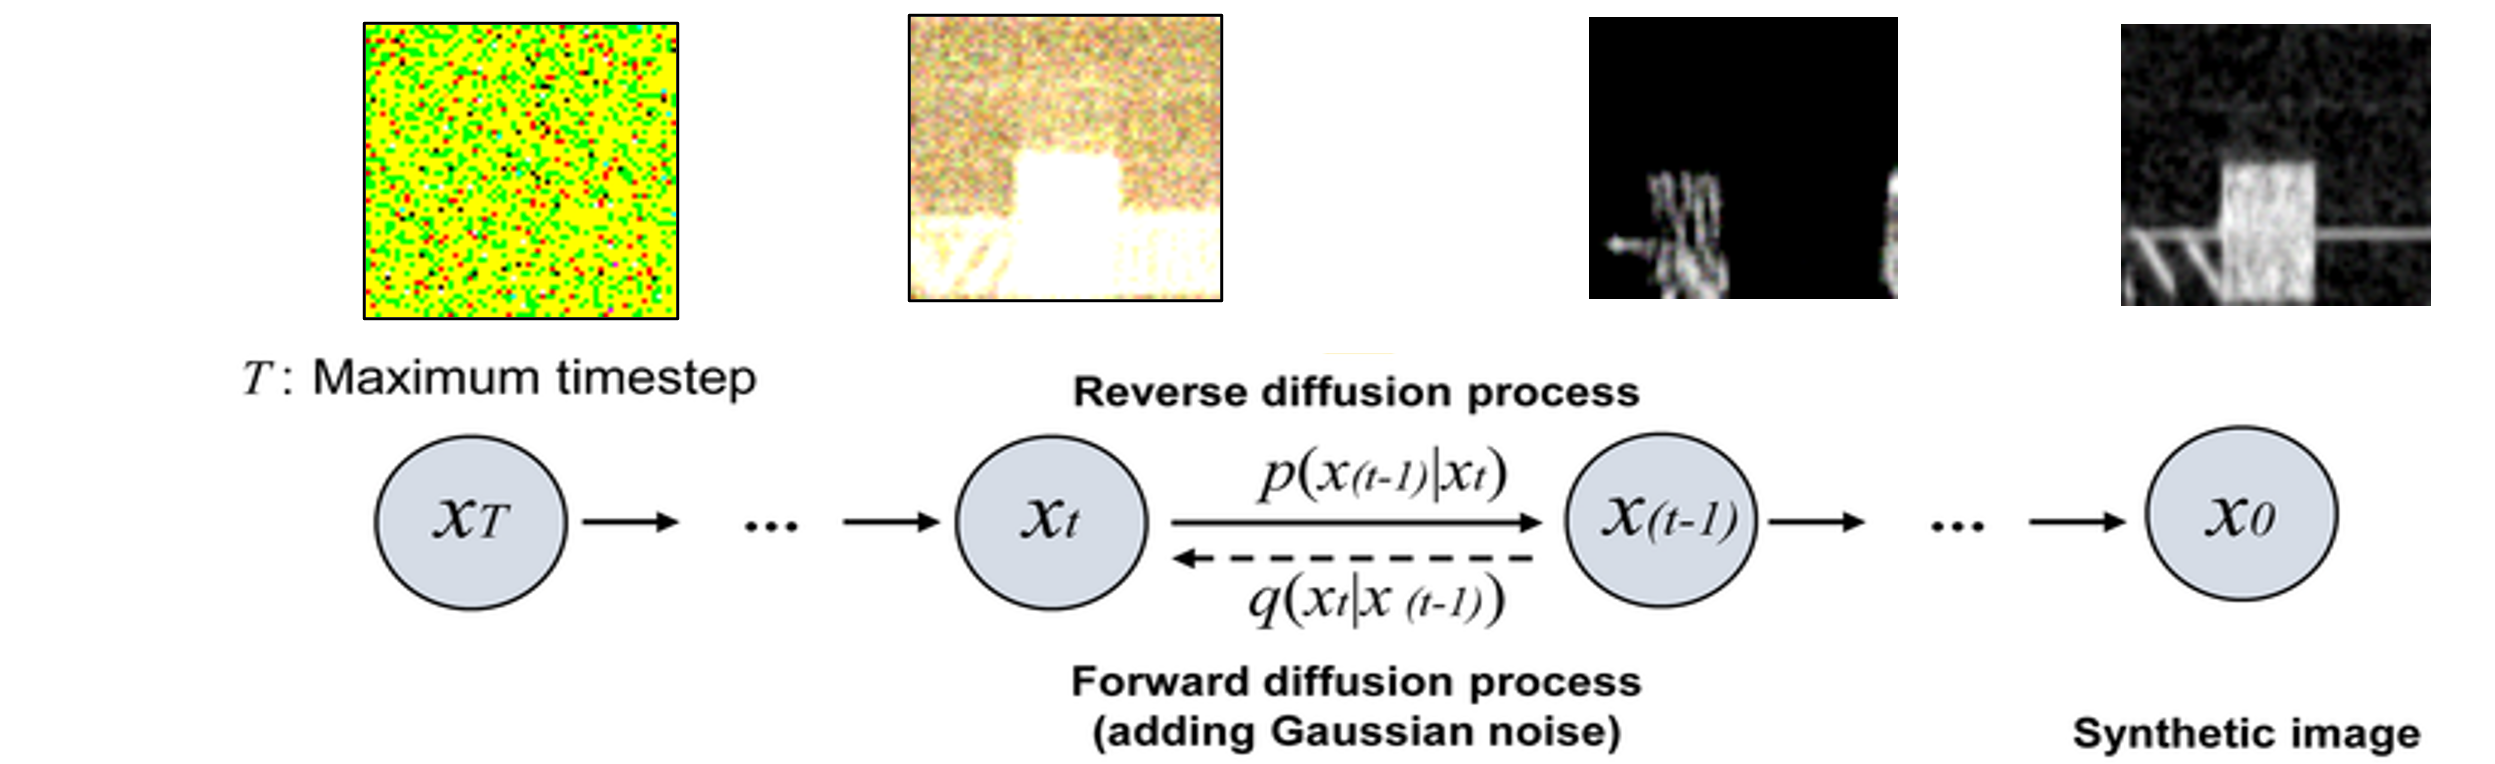
\includegraphics[width=\textwidth]{figures/ddpm.png}
\centering
\caption{ Diffusion process of the \gls{ddpm}}
\centering
\end{figure}

During the forward process, the clean image $y_0$ is sampled with Gaussian noise of variance ${\beta_1,....,\beta_T}$ is added over $T$ time steps.
\begin{equation}
\begin{split}
    q(y_t\mid y_0) :=\mathcal{N}(y_t;\sqrt{\bar{\alpha_t}}y_0,(1-\bar{\alpha_t})I)\\
    =\sqrt{\bar{\alpha_t}}y_0+\epsilon\sqrt{1-\bar{\alpha_t}},\epsilon \sim \mathcal{N}(0,I)
    \end{split}
\end{equation}
Where $\alpha_t=1-\beta_t$

In the reverse process, the added noise is removed step by step to recover the image $y_0$.
\begin{equation}
    p(y_T)=\mathcal{N}(0,I)
\end{equation}
\begin{equation}
    p(y_{(t-1)}\mid y_t)=\mathcal{N}(y_{(t-1)};\mu_{\theta}(y_t,t),\sqrt{\beta_t}I)
\end{equation}

We used a conditional \gls{ddpm}, and when training the \gls{ddpm} we enabled mixed precision training and multithreaded data loaders. We sampled the images regularly during the training and we could see the learning rate gradually decreasing with the time steps. 
For training our model we sampled a timestep $t\sim U[1,T]$ with $T=2000$ and a $5\times10^{-3}$ learning rate.
After training the model, we used the trained weights to generate 1200 images with 100 images per class and used the pre-trained \gls{cnn} model to classify the images to their respective classes. 
\begin{figure}[h]
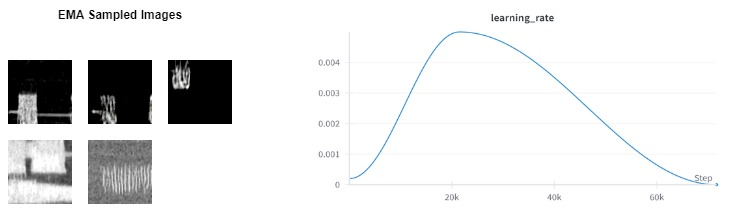
\includegraphics[width=\textwidth]{figures/ema_learning_rate.jpg}
\centering
\caption{EMA sampled images and the change of the learning rate with each time step when training the \gls{ddpm} }
\centering
\end{figure}
%%%%%%%%%%%%%%%%%%%%%%%%%%%%%%%%%%%%%%%%%%%%%%%%%%%%%%%%%%%%%%%%%%%%%%%%%%%%%%%%%%%%%%%%%%%%%%%%%
\section{\gls{cnn}}
\gls{cnn}s are a class of deep learning models commonly used for analyzing images. They automatically learn spatial feature hierarchies from input data by applying multiple layers of convolutional filters.
These filters detect patterns such as edges, textures, and more complex features in the images, making \gls{cnn}s highly effective for tasks like image classification.


We trained a \gls{cnn} model that can detect collision scenarios using the generated spectrogram data from the three models. 
Since the spectrogram images generated by the \gls{ddpm}, \gls{gan}, and \gls{vq-vae} models contained some noise, which could have led to misclassification by conventional \gls{cnn} architectures, particularly when distinguishing fine-grained features,  we employed an enhanced \gls{cnn} architecture specifically designed to effectively capture and differentiate subtle details within the images, thereby mitigating the impact of noise on classification accuracy.

We used a \gls{cnn} architecture based on a modified ResNet-50 model, enhanced with a \gls{cbam} to improve its feature extraction and classification capabilities. The architecture comprised convolutional layers for basic feature extraction, residual blocks for efficient gradient propagation, \gls{gap} for summarizing spatial information, and a \gls{fc} layer adapted for classifying the 12 spectrogram image classes.

The model was trained on spectrogram images resized to 448×448 for capturing finer details. The training used the Adam\cite{18} optimizer for adaptive gradient updates and a learning rate scheduler that reduced the learning rate every five epochs to ensure stable convergence.  

%%%%%%%%%%%%%%%%%%%%%%%%%%%%%%%%%%%%%%%%%%%%%%%%%%%%%%%%%%%%%%%%%%%%%%%%%%%%%%%%%%%%%%%%%%%%%%%%%
\section{\gls{drl}}

In this work, we employed a \gls{drl} agent to learn optimal spectrum access strategies in a simulated \gls{cbrs} environment. The agent interacts with an environment that mimics the dynamic characteristics of the CBRS band, including incumbent radar signals and LTE-based priority access users. The environment is modeled as a Markov Decision Process (MDP) where the agent observes the occupancy of two communication channels and selects an action from a discrete set: idle, use channel 1, or use channel 2.

We implemented a \gls{dqn} agent that approximates the Q-value function using a neural network. The agent receives as input a two-dimensional observation vector representing the current channel state, where each element indicates whether a channel is occupied (1) or free (0), as predicted by the pre-trained \gls{cnn} model that analyzes the spectrogram of the received signal. The agent’s goal is to maximize a cumulative reward by learning a policy that avoids interference with higher-tier users while efficiently utilizing the available spectrum. The reward structure is defined such that selecting an idle channel yields a positive reward, selecting an occupied channel results in a penalty, and remaining idle results in a small negative reward to discourage inactivity.

The neural network used by the DQN agent consists of a feature input layer followed by two fully connected layers with ReLU activations, and a final output layer that estimates Q-values for each possible action. During training, we enabled GPU acceleration to improve performance. The training utilized an experience replay buffer and a target network, and was configured with Double DQN and a smooth target update factor of $10^{-3}$ to stabilize learning. We set the discount factor $\gamma=0.99$, and trained the model for 1000 episodes with a maximum of 100 steps per episode.

The environment generates new signal observations by randomly simulating different channel conditions, including ‘empty’, ‘radar’, ‘LTE’, and ‘collision’. These synthetic signals are converted into spectrogram images, resized to 224$\times$224 pixels, and classified by the CNN. This predicted class is used to update the channel occupancy vector, which forms the observation space for the DRL agent.

%%%%%%%%%%%%%%%%%%%%%%%%%%%%%%%%%%%%%%%%%%%%%%%%%%%%%%%%%%%%%%%%%%%%%%%%%%%%%%%%%%%%%%%%%%%%%%%%%
\section{System Architecture}

We evaluated classification performance across different generative models and computed class-wise and overall accuracy, along with \gls{fid} scores for each class. Then, we used a pre-trained CNN model trained with a dataset comprising both original data and the data generated by the three generative models to detect incumbent users. Figure 2.7 illustrates this scenario.
\begin{figure}[h]
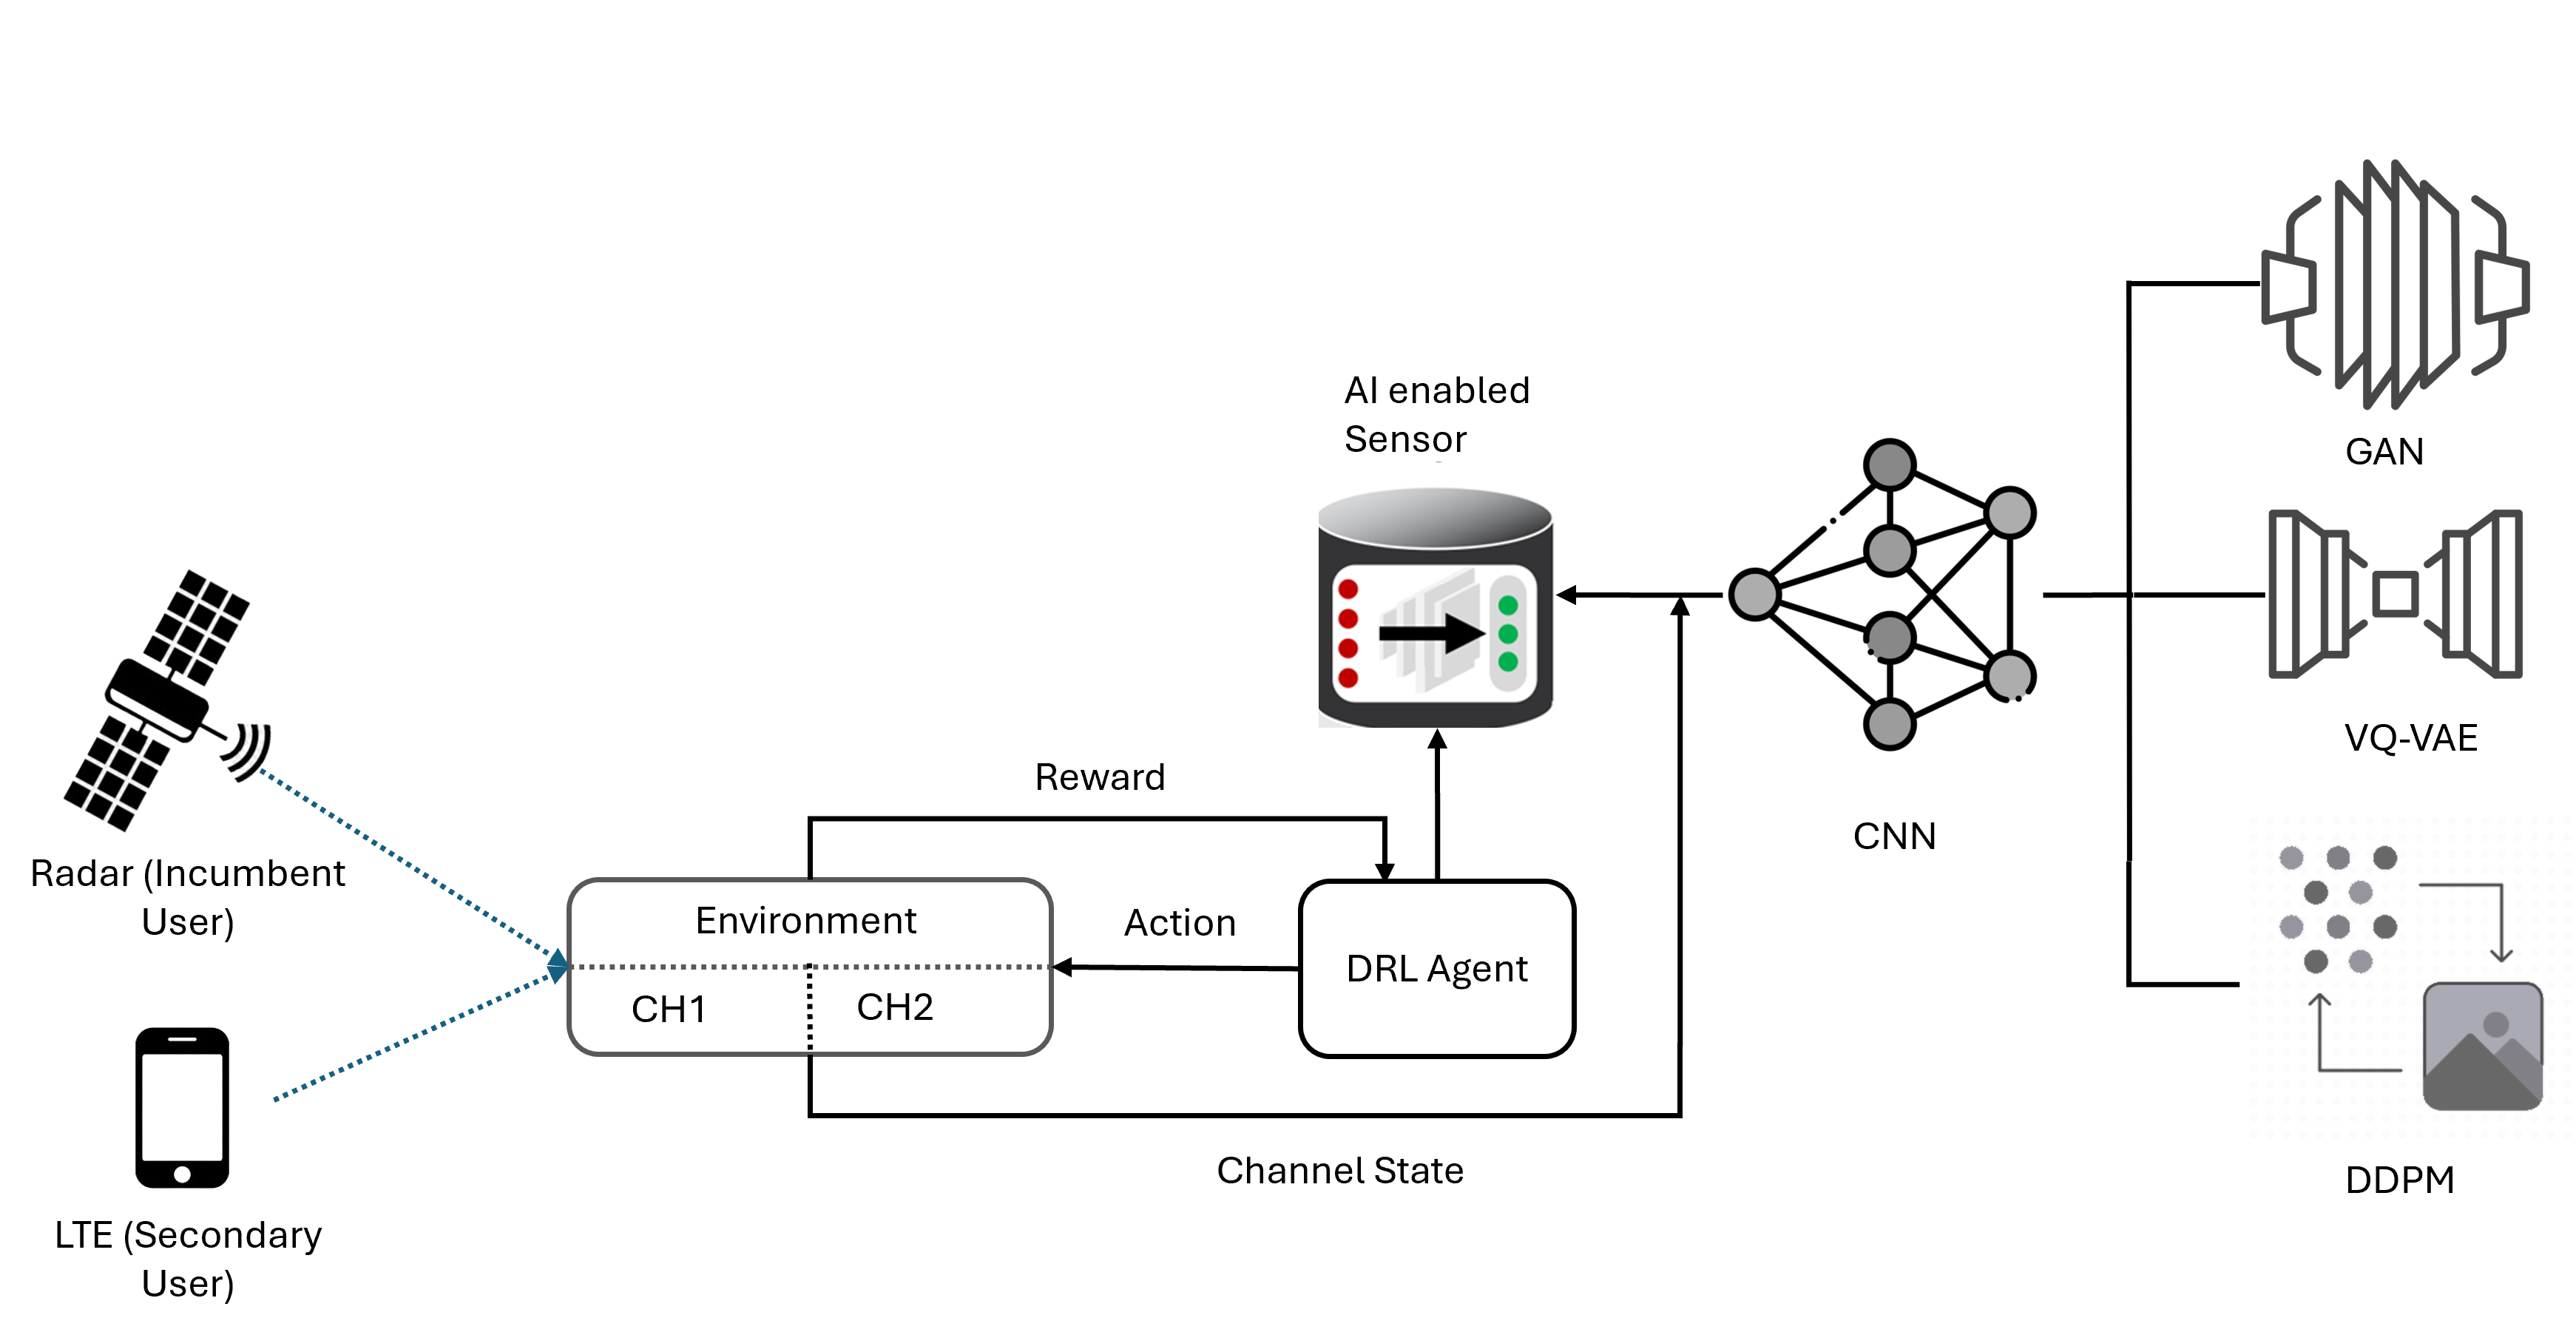
\includegraphics[width=\textwidth]{figures/system-architecture.png}
\centering
\caption{ System Architecture}
\centering
\end{figure}

\section{Experimental Setting}
\subsection{\gls{vq-vae}}
The conditional \gls{vq-vae} model was designed for class-specific image generation, with an encoder that compresses grayscale inputs through three convolutional layers and residual blocks to enhance feature extraction. The quantization layer, class-conditioned, uses a codebook of 512 embeddings (64 dimensions each) to discretize the latent space. A 1×1 convolution adjusts the encoder's output to fit the quantizer's input requirements. The decoder, structured similarly to the encoder, uses transposed convolutions and residual stacks to reconstruct high-fidelity images from quantized representations. The model generated 1,200 images, with 100 per class across 12 classes, which were classified using a pre-trained \gls{cnn}.

\subsection{\gls{gan}}
The conditional \gls{gan} used in this study consists of a generator and discriminator trained in a min-max game. The generator takes a 100-dimensional noise vector and class embeddings, passing them through five convolutional layers with ReLU activations and a Tanh output to generate pixel values in the range [-1, 1]. The discriminator uses five convolutional layers with Leaky ReLU activations to downsample input images, and a Sigmoid output provides a probability score. The model generated 1,200 images, with 100 per class across 12 classes, which were classified using a pre-trained \gls{cnn}.

\subsection{\gls{ddpm}}
The conditional \gls{ddpm} used in this study generates images through a two-stage Markovian process: a forward process, where Gaussian noise is added to the clean image over T=2000 timesteps, and a reverse process, where the model removes the noise step-by-step to reconstruct the original image. Mixed precision training and multithreaded data loaders were utilized for efficiency, and images were sampled during training to monitor progress. The model was trained with a learning rate of $5\times10^{-3}$, sampling timesteps $t\sim U[1,T]$ After training, 1,200 images (100 per class) were generated and classified using a pre-trained \gls{cnn}.

\subsection{\gls{cnn}}
A modified ResNet-50 architecture with a \gls{cbam} was used to classify 12 spectrogram image classes, effectively capturing fine-grained details despite noise. The model was trained on 448×448 resized images using the Adam optimizer and a learning rate scheduler to ensure stable convergence. For training, we used a combination of the original dataset and the generated data from each model. The combined dataset was divided into 80\% for training and 20\% for inference, and the results are based on three separately trained models, each incorporating generated data from one of the three-generation models.

We compared the class-wise and overall accuracy of the \gls{cnn} classification model trained with data generated by different models for the inference set. Then, we calculated the \gls{fid} score for each class. 

\subsection{\gls{fid}}
\gls{fid} is a widely used metric for evaluating the quality of images generated by generative models. It quantitatively compares the distributions of features extracted from real and generated images in a high-level feature space. These features are typically obtained from a pre-trained neural network, such as the Inception-v3 model. The \gls{fid} score is lower when the two distributions are closer, indicating higher quality and diversity of the generated images [21].

Let $\mu_r$ and $\Sigma_r$ represent the mean and covariance of the features extracted from real images, and $\mu_g$ and $\Sigma_g$ represent the mean and covariance of the features extracted from generated images. The \gls{fid} score is calculated using the following formula:

\begin{equation}
\text{FID} = \|\mu_r - \mu_g\|_2^2 + \text{Tr}(\Sigma_r + \Sigma_g - 2 (\Sigma_r \Sigma_g)^{\frac{1}{2}})
\end{equation}

Usually, to compute the \gls{fid}, real and generated images are passed through the pre-trained Inception-v3 network, and features are extracted from a specific layer (often the "pool3" layer). The means and covariances of these features are then computed for both datasets. However, in this paper, we used a ResNet18 model with the final classification layer replaced instead of Inception-v3.  The ResNet18 model employed for \gls{fid} calculation is distinct from the \gls{cnn} model used for classification. While the ResNet18 was trained exclusively on the original dataset to extract consistent feature representations for real and generated images, the classification \gls{cnn} was trained on a combined dataset comprising both real and synthetic data. This separation ensures that the \gls{fid} evaluation remains unbiased by the influence of synthetic data used in the classification task. Finally, the \gls{fid} score is calculated by substituting these statistics into equation 2.7. 

A lower \gls{fid} Score indicates that the distributions of real and generated features are more similar, implying better quality and diversity of generated images whereas a higher \gls{fid} score indicates that the generated images are less similar to real images, suggesting poorer quality or lack of diversity.

\subsection{\gls{pca}}
\gls{pca} is a statistical technique used for dimensionality reduction, facilitating the analysis and visualization of high-dimensional data. By transforming the original variables into a new set of uncorrelated variables, \gls{pca} captures the directions of maximum variance in the data. The first principal component accounts for the largest possible variance, with each succeeding component accounting for the remaining variance under the constraint of being orthogonal to the preceding components. This method simplifies complex datasets while preserving their essential patterns and structures \cite{12}.

\subsection{\gls{drl}}
The \gls{drl} agent observes the current state (e.g., channel occupancy or spectrogram predictions), selects an action (e.g., choose Channel 1, Channel 2, or remain idle), and receives a reward based on the outcome (e.g., successful transmission or interference avoidance). Over repeated episodes, the agent learns to maximize its long-term performance, such as throughput or interference avoidance, by training a neural network to approximate optimal policies. Figure 2.8 depicts Incumbent signals generated by the MATLAB simulation, where the agent learns to select the best channel based on the spectrogram images generated by the three models. The agent's training involved 1000 episodes, with each episode consisting of 100 steps, and it was trained using a reward structure that incentivized efficient spectrum access while avoiding interference with higher-tier users.
The agen was rewarded or penalized according to the steps it chose to take. The reward structure was defined as shown in Table 2.1.
\begin{table}[ht]
    \centering
    \caption{DRL agent reward structure}
    \begin{tabular}{| c | c | c|}
    \hline
    \textbf{Action} & \textbf{Channel State} & \textbf{Reward} \\
    \hline
    Idle (0) & Both channels empty & -0.1 \\
    Idle (0) & Any channel non-empty (primary or collision) & +0.2 \\
    Use CH1(1) & CH1 Empty & +1.0 \\
    Use CH1(1) & CH1 Primary & -2.0  \\
    Use CH1(1) & CH1 Collision  & -1.5  \\
    Use CH1(1) & CH1 Secondary & +0.5 \\ 
    Use CH2(2) & CH2 Empty & +1.0  \\ 
    Use CH2(2) & CH2 Primary & -2.0  \\
    Use CH2(2) & CH2 Collision & -1.5  \\
    Use CH2(2) & CH2 Secondary & +0.5  \\
    
    \hline
    \end{tabular}
    \label{tab:scenario_labels}
\end{table}
    
    The agent was highly rewarded for choosing an empty channel and penalized for choosing a channel occupied by a primary user. The agent was also rewarded for using a secondary channel, but less than when it chose an empty channel. The agent was penalized for choosing a channel occupied by a collision or primary user. The agent was also penalized for remaining idle, but less than when it chose a channel occupied by a primary user.

\begin{figure}[h]
    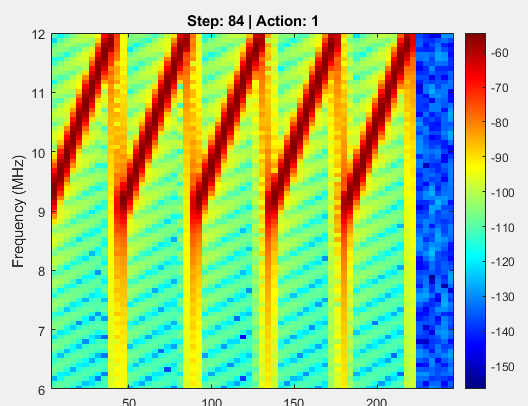
\includegraphics[width=0.5\textwidth]{figures/matlab_simulation.png}
    \centering
    \caption{ Spectrograms of the signals generated by the simulated CBRS environment in MATLAB}
    \centering
\end{figure}
    